
\begin{figure}[htbp]
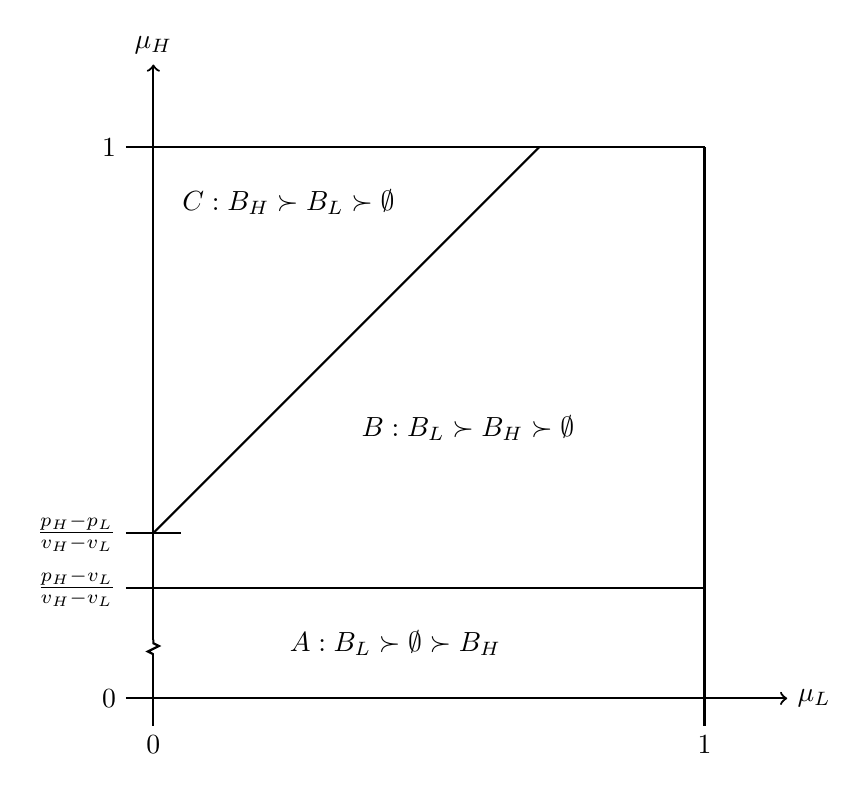
\begin{tikzpicture}[scale=7]
\draw[thick,->] (-0.05,0) -- (1.15,0) node[anchor=west] {$\mu_L$};
\draw[thick] (0,-0.05) -- (0,0.08);
\draw[thick,->] (0,0.1067) -- (0,1.15) node[anchor=south] {$\mu_H$};
\draw[thick] (-0.05,1)--(1,1);
\draw[thick] (1,1)--(1,-0.05);
\draw[thick] (-0.05,0.2)--(1,0.2);
\draw[thick] (0,0.3)--(0.7,1);
\draw[thick] (-0.05,0.3)--(0.05,0.3);

\node[left] at (-0.05,0) {0};
\node[left] at (-0.05,1) {1};
\node[below] at (0,-0.05) {0};
\node[below] at (1,-0.05) {1};
\node[left] at (-0.05,0.2) {$\frac{p_H-v_L}{v_H-v_L}$};
\node[left] at (-0.05,0.3) {$\frac{p_H-p_L}{v_H-v_L}$};

\node[right] at (0.035,0.9) {$C: B_H \succ B_L \succ \emptyset$};
\node[right] at (0.36,0.49) {$B: B_L \succ B_H \succ \emptyset$};
\node[right] at (0.23,0.1) {$A: B_L \succ \emptyset \succ B_H$};
\draw[decorate,decoration={zigzag,amplitude=2pt,segment length=4pt},thick] (0,0.08) -- (0,0.1067);
\end{tikzpicture}
\caption{Buyer Belief Space}
\label{belief_space}
\end{figure}
